\section{Redes Neuronales}

\subsection{Brevísima historia}
\subsection{Definición}
\subsection{Multi-layer perceptron}

Una red neuronal puede pensarse simplemente como una función $f: \mathbb{R}^m \rightarrow O$ que intenta aproximar una función $f^*$ con misma aridad. Podremos notar $ y = f(x; \Theta)$, siendo $\Theta$ los parámetros de dicha función

El perceptrón, desarrollado en 1958 por Frank Rosenblatt \cite{rosenblatt1958perceptron}, intenta ajustar

\begin{equation*}
    y = H(\Theta_1 x + \Theta_0)
\end{equation*}

donde $H$ es la función de activación, y $\Theta = (\Theta_0, \Theta_1)$ son los parámetros de la función. Este modelo es el primero cuyos pesos se encontraban mediante un algoritmo, considerando que $H$ es una función derivable. Este puede considerarse como el primer modelo de una neurona, junto al modelo de McCulloch-Pitts.

\citet{minsky1969perceptrons} demostraron que este tipo de modelos sólo pueden ajustarse a datos linealmente separables, provocando el primer ``invierno'' de las redes neuronales.

Una forma de sortear estas dificultades planteadas es ``apilar'' (stack en inglés) varias de estas funciones para poder ajustar a más tipos de funciones. En términos matemáticos, esto es tan sólo una composición de funciones, tomando ahora $f = f_3 \circ f_2 \circ f_1$, donde $f_1$ es la primer ``capa'' de nuestra función correspondiente a la entrada, $f_2$ es la capa intermedia u oculta, y $f_3$ es la capa de salida. Si bien este ejemplo consta de 3 capas, se puede generalizar a arbitrarias capas ocultas. Este modelo es el que conocemos como \textbf{Perceptrón Multicapa} o \textbf{Multi-Layer Perceptron} (MLP por sus siglas en inglés)






\subsection{Redes neuronales recurrentes}

Los problemas descriptos de NLP suelen constar de procesar una secuencia de palabras o tokens $x_1, x_2, \ldots, x_k$ de longitud variable, de manera de ajustar a una función

\begin{equation*}
    y = f([x_1, \ldots, x_k])
\end{equation*}

Una manera de ajustar una función de este tipo (usando una entrada de largo fijo) es convertir este problema a ajustar una función autorregresiva

\begin{equation*}
    y_k = f(x_k, y_{k-1})
\end{equation*}

donde tenemos una salida para cada paso $k$ de tiempo. Si $f$ es una red neuronal, llamamos a este tipo de redes neuronales \textbf{recurrentes}, ya que la salida a cada paso ($y_k$) depende de la salida del paso anterior, $y_{k-1}$\footnote{No confundir con las redes neuronales recursivas}.

Una primer aproximación a este problema es la red recurrente de Elman \cite{elman1990finding} definida por las siguientes ecuaciones

\begin{align}
h_t &= \sigma(W_h x_t + U_h h_{t-1} + b_h) \\
y_t &= \sigma(W_y h_t + b_y)
\label{eq:elman}
\end{align}

$h_t$ es normalmente llamado el \textbf{estado oculto} en las redes neuronales recurrentes. Los parámetros a ajustar son $W_h, U_h$ (matrices) y $b_h, b_y$ (escalares). Podemos ver que, a grandes rasgos, este tipo de red recurrente no es nada más que un perceptrón multicapa cuya entrada consta de $x_t$, la entrada original en el tiempo actual $t$, y el estado oculto anterior, $h_{t-1}$.

Para entrenar este tipo de redes recurrentes utilizamos back-propagation through time (BPTT), que consta en desplegar la relación recurrente y aplicar back-propagation de manera normal. \todo{explicar un poco mejor esto}

Este tipo de redes recurrentes sufren de varios problemas: entre ellos, \textbf{vanishing gradient} y \textbf{exploding gradient}. Estos problemas pueden observarse ya que el cálculo del gradiente de las ecuaciones \ref{eq:elman} usando BPTT induce la potencia a la $n$ (donde $n$ es el largo de la secuencia) de las matrices $W_h$ y $U_h$. Usando la descomposición de Jordan de estas matrices, podemos ver que sus elementos en la diagonal que sean distintos de 1, o bien tienden a infinito o a cero.

El problema de \textbf{exploding gradient} puede solucionarse mediante la técnica de \textbf{gradient clipping}\todo{citation needed}, que consta de reajustar la norma del gradiente. Sin embargo, nos queda aún el problema de \textbf{vanishing gradient}. Para ello, se han propuesto otras arquitecturas recurrentes.

\citet{hochreiter1997long} propusieron las \textbf{Long Short-Term Memory} (LSTM) como solución a estos problemas. Para solucionar los problemas mencionados, proponen una arquitectura basadas en compuertas (\textbf{gates}) que regulan los cambios en el estado oculto y en la salida. Concretamente, la arquitectura de las LSTMs está regida por las siguientes ecuaciones\footnote{Para una muy buena explicación de las redes recurrentes, sugerimos este artículo: \url{https://colah.github.io/posts/2015-08-Understanding-LSTMs/}}:


\begin{align}
    h_t &= \sigma(W_h x_t + U_h h_{t-1} + b_h) \\
    y_t &= \sigma(W_y h_t + b_y)
    \label{eq:lstm}
\end{align}



\subsection{Optimización}


\section{Técnicas de representación de NLP}
\subsection{Word-embeddings}



\subsubsection{Sub-word embeddings}

\subsection{Modelos pre-entrenados}

\subsection{BERT}
\label{sec:02_preliminar_bert}

\subsubsection{Transfer Learning}

\subsection{ELMo}
% \begin{figure}
%     \centering
%     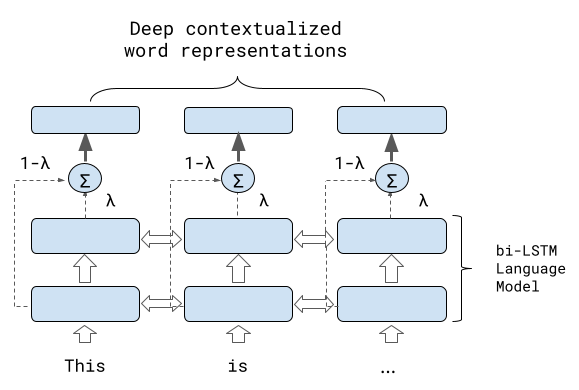
\includegraphics[width=0.65\textwidth]{img/ELMo.png}
%     \caption{Ilustración de ELMo. Las dos capas inferiores representan un modelo de lenguaje bidireccional, y la superior representa una combinación lineal convexa de las salidas de las capas recurrentes}
%     \label{fig:modelos_offenseval_hateval}
% \end{figure}
\subsection{ULM-Fit}
\subsection{BERT}